\documentclass[a4j,openany]{jbook}
\usepackage{ascmac}
\usepackage[dvipdfmx]{graphicx}
\usepackage[dvipdfm,bookmarkstype=toc=true,colorlinks=true,urlcolor=blue,linkcolor=blue,citecolor=blue,linktocpage=true,bookmarks=false]{hyperref}

\usepackage{color}
%\usepackage{graphicx}
\usepackage{verbatim}

\usepackage{supertabular}
\usepackage{longtable}

\title{{\Huge \textbf{Akiraの手引書}}\\ }
\author{中村貴英}
\date{\today}

\setcounter{tocdepth}{2}

\begin{document}
\maketitle
\frontmatter
\chapter{はじめに}
可視化ツールAkiraのマニュアルです.
この文章は中村貴英によって書かれました.よって文責は中村貴英にあります.

\tableofcontents
\mainmatter

\chapter{Akiraとは}
Akiraとは計算機シミュレーションの結果を可視化するソフトウエアです.
もともとは尾形先生の先輩である中野先生の研究室で,C言語とOpenGL(glut)を使って開発
されたatoms viewerというソフトウエアが起源となっています.
このatoms viewerを河野さんがJAVAに移植しKVS(Kouno Viewer System)の名前で
しばらく使われていました.
それをもとに中村がフルスクラッチで書き直し,現在に至ります.
現在は,名古屋工業大学の尾形研の有志によって改良・保守されています.

またAkiraはJAVAとOpenGLによって作られています.
これは
\begin{enumerate}
 \item JAVAが,プラットホームに依存せず実行できること
 \item JAVAが,多人数での開発に向いていると言われている
       オブジェクト指向を体現した言語であること
 \item OpenGLが,描画ライブラリとして一般的で情報が得やすいこと
\end{enumerate}
を理由としています.

 \section{Akiraの構成}
 Akiraでは,描画時の高速化の為にデータを一旦Akira専用のバイナリに変換します.
 その為AkiraはConverterとViewerの二つからなります.
 \begin{figure}[htbp]
  \begin{center}
   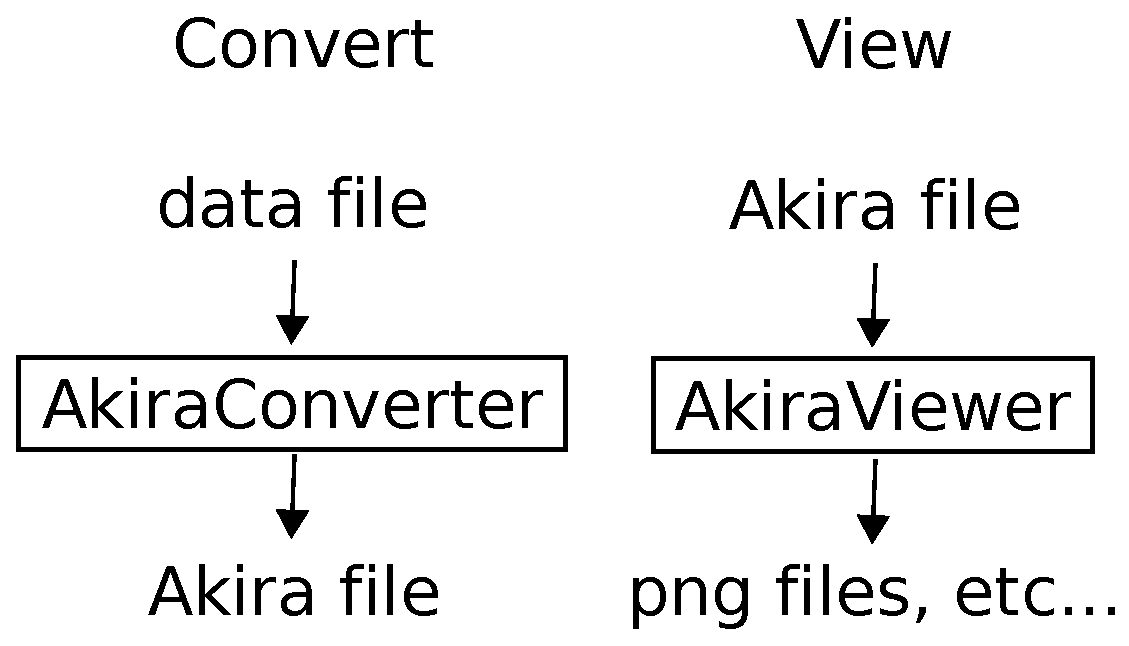
\includegraphics[width=8cm]{img/flow.eps}
  \end{center}
  \caption{Akiraで可視化するまで}
 \end{figure}

  \subsection*{AkiraConverter}
 描画に必要なデータのみを集約し,バイナリファイルとして保存します.
 読み込みファイルのフォーマットは Sec.\ref{sec:Akira-format}を参照してください.

  \subsection*{AkiraViewer}
 AkiraConverterで変換されたAkiraファイル(拡張子は.Akira)を読み込んで表示します.
 Viewerの設定ファイルは,\~{}/.Akira/またはC:Akiraに保存されます.

 \section{Akiraの遍歴}
\begin{description}
 \item[2008以前]
            atomsviewerが使われる
 \item[2008-12-04]
            KVS開発スタート
 \item[2009-07-08]
            KVS開発終了.KVS2開発スタート
 \item[2010-11-28]
            外部公開に向けて,KVSからAkiraへ改名.
            マニュアル整備.
 \item[2010-12-26]
            ホスティングサーバーをGoogle Project Hostingへ.
\end{description}
\chapter{インストール方法}
AkiraはJOGL(\htmladdnormallink{http://jogamp.org}{http://jogamp.org})
とJAVAがあれば動きます.
JOGLとはOpenGLをJAVAから使う為のライブラリです.
JAVAは大抵の環境でインストール済みと思われるので,
JOGLのみ新たにインストールする必要があります.
Akiraはjarファイル(JAVAの実行形式)で配布されます.
Akiraの最新版は
\htmladdnormallink{http://code.google.com/p/project-akira/downloads/list}
{http://code.google.com/p/project-akira/downloads/list}
からダウンロード可能です.
インストールは
\begin{itemize}
 \item JOGLの設置,および設置したディレクトリにPATHを通す
 \item Akira.jarの設置
 \item Akira.jarを呼び出すスクリプトの設置
\end{itemize}
を行うのみです.
アップデートがある場合,Akira.jarを入れ替えるのみで,JOGLを入れ替える必要はありません.

 \section{Mac OSX/Linuxの場合}
 このセクションではJOGLを\verb|~/myLocal/javalib/jogl|に,
 Akira.jarを\verb|~/myLocal/Akira/|に置くとして
 話を進めます.
 \footnote{これらのディレクトリが気に入らない上級者は,自由に変更して下さい.
 ただしAkiraの設定ファイルの置き場所は,\~{}/.Akira/で固定なので注意して下さい.}

  \subsection{準備}
  以下を実行してディレクトリを作っておきます.
   \begin{screen}
\begin{verbatim}
mkdir ~/myLocal
mkdir ~/myLocal/bin
mkdir ~/myLocal/javalib
mkdir ~/myLocal/javalib/jogl
mkdir ~/myLocal/Akira
mkdir ~/.Akira
\end{verbatim}
   \end{screen}

また以下を.bashrcに書き込みます.
    \begin{screen}
\begin{verbatim}
export JOGL_LIB=~/myLocal/javalib/jogl
export DYLD_LIBRARY_PATH=$JOGL_LIB:$DYLD_LIBRARY_PATH
export LD_LIBRARY_PATH=$JOGL_LIB:$LD_LIBRARY_PATH
export PATH=$PATH:~/myLocal/bin
\end{verbatim}
    \end{screen}
また以下を.bash\_profile
    \begin{screen}
\begin{verbatim}
source ~/.bashrc
\end{verbatim}
    \end{screen}
に書きこんで,ターミナルを再起動して,設定を反映させます.

  \subsection{JAVAのインストール}
  Mac OSXの場合,標準でJAVAがインストールされています.
  むしろ,画面左上リンゴマーク-ソフトウエアアップデートで最新版にして下さい.
  Linuxを使う人はエキスパートと思われるので,各自インストールを行ってください.

  \subsection{JOGLのインストール}
  \htmladdnormallink{http://download.java.net/media/jogl/builds/archive/jsr-231-2.0-beta10/}
  {http://download.java.net/media/jogl/builds/archive/jsr-231-2.0-beta10/}
  からJOGL
  \footnote{
  64bit CPUのLinuxの人はjogl-2.0-linux-amd64.zip,
  32bit CPUのLinuxの人はjogl-2.0-linux-i586.zip,
  Mac OSXの人はjogl-2.0-macosx-universal.zipです.
  }
  をダウンロードします.
  解凍し,libの中身を\verb|~/myLocal/javalib/jogl|に置いて下さい.
  \footnote{
  OSXの場合は環境変数{\bf DYLD\_LIBRARY\_PATH},
  Linuxの場合は環境変数{\bf LD\_LIBRARY\_PATH}に
  \~{}/myLocal/javalib/joglを設定します.
  が,準備でこれらの設定は済んでいます.
  }
  \subsection{Akira.jarのインストール}
  Akira.jarを\verb|~/myLocal/Akira/|に置いて下さい.
  \footnote{Akiraのアップデートは,\~{}/myLocal/Akira/にあるAkira.jarを入れ替えることで完了します}
  \subsection{シェルスクリプトのインストール}
  自分のプラットホームにあわせたshell-script-***の中身を\verb|~/myLocal/bin/|に置きます.


  \subsection{動作確認}
  \htmladdnormallink{http://project-akira.googlecode.com/files/sample.zip}
  {http://project-akira.googlecode.com/files/sample.zip}
  からsample.zip
  をダウンロード,解凍してその中で以下を実行します.
   \begin{screen}
\begin{verbatim}
Akira.sh
\end{verbatim}
   \end{screen}
   問題なく表示されれば,インストールは完了です.
   うまく表示されない場合はエラー文を参考に問題解決してください.

 \section{Windowsの場合}
 {\bf windowsにおいて,Akiraの設定ファイルはC:Akiraに保存されます.
 故にディレクトリC:Akiraは必須です.}
 windowsでは,Akira.jarもC:Akiraに置く事を推奨します.
 尚,JOGLはC:joglに置くとして話を進めますが,JOGLの置き場所は自由です.

 またwindowsに疎い人間が書いている文章なので,
 もっとスマートな設定方法があれば教えてください.

  \subsection{準備}
  Cドライブの直下に
  joglおよびAkiraという名前のフォルダを作っておいて下さい.

  \subsection{JAVAのインストール}
  JREをインストールしてください.

  \subsection{JOGLのインストール}
  まずCドライブの直下にjoglというフォルダを作ります.
  そして
  \htmladdnormallink{http://download.java.net/media/jogl/builds/archive/jsr-231-2.0-beta10/}
  {http://download.java.net/media/jogl/builds/archive/jsr-231-2.0-beta10/}
  からJOGL
  \footnote{64bit CPUを使っている人はjogl-2.0-windows-amd64.zip,
  32bit CPUを使っている人はjogl-2.0-windows-i586.zipです.}
  をダウンロードします.
  解凍して,libの中身をC:joglに置いて下さい.

   更にコントロールパネル-システム-詳細設定-環境変数にて,PATHに
   \begin{screen}
\begin{verbatim}
C:jogl
\end{verbatim}
   \end{screen}
   を追加します.

  \subsection{Akira.jarのインストール}
  Cドライブの直下にAkiraというフォルダを作ります.
  そしてAkira.jarをC:Akiraに置いて下さい
  \footnote{Akiraのアップデートは,C:AkiraにあるAkira.jarを入れ替えることで完了します}
  .
  {\bf Akiraの設定ファイルをC:Akiraに保存する様にプログラムされている為,
  このディレクトリが無ければ正常に動作しません.}

  \subsection{バッチファイルのインストール}
  お好きなところへ置いて下さい.

  \subsection{動作確認}
  \htmladdnormallink{http://project-akira.googlecode.com/files/sample.zip}
  {http://project-akira.googlecode.com/files/sample.zip}
  からsample.zip
  をダウンロード,解凍してその中で以下を実行します.
   \begin{screen}
\begin{verbatim}
AkiraConverter.bat
AkiraViewer.bat
\end{verbatim}
   \end{screen}

\chapter{Converterの詳細}
現在,AkiraConverterでは
 \begin{itemize}
  \item Akiraフォーマット
  \item CHGCAR
  \item Gaussian cube
 \end{itemize}
 を読み込むことが出来ます.

 \section{Akiraフォーマットについて}\label{sec:Akira-format}
 Akiraフォーマットを出力するサンプルコードを
  Fig.\ref{fig:akira-ascii}および
  Fig.\ref{fig:akira-binary}に示します.
  これらはtar.gz
  \footnote{\tt tar czvf a.tgz out*}
  tar.bz2
  \footnote{\tt tar cjvf a.tbz2 out*}
  で形式で圧縮されているならば,解凍する事無く読み出しが可能です.

\chapter{Viewerの詳細}
AkiraConvにて変換された,専用のAkiraファイル(拡張子は.Akira)を読み込んで表示します.

 \section{機能一覧}
  \subsection*{原子を点,球で描く}
   最も早い描画は点で描くことです.
   また最終的には球で描くと思います.
   その場合は,緯度と経度方向のスライスを指定して球の滑らかさを決定します.
   もちろんスライスが増えるに連れて,描画は遅くなります.
   それらはatomsパネルで指定します.
   またそれぞれの原子が持つデータを基に,色を決定するモードもあります.

  \subsection*{ボンドを線,円筒で描く}
   これもやはり早い描画は線で描くときです.

  \subsection*{ベクトル}
   任意のベクトル量を矢印として描画出来ます

  \subsection*{ライトの設定}

  \subsection*{背景色,文字色などの設定}
   印刷する場合は背景色を白にした方が,インクの節約になるでしょう.

  \subsection*{View pointの保存}
  現在の視点を保存することが可能です.
  次回のAkira起動時に同じ視点が再現出来ます.

  \subsection*{静止画像として出力(png,jpg,bmp)}
  デフォルトではpng形式で出力します.
  各フレームを画像ファイルに出力し,連結すればムービーが出来上がります.

  \subsection*{任意の面でカット可能}
  任意の面でカットして,断面を見ることが可能です.
  面の指定は,その法線ベクトルと面が通る点を指定することで行います.

  \subsection*{Volume Rendering}
  additional dataは原子一つ一つのデータであるのでバラツキが大きく,
  なんらかの平均をしなければ,見るに耐えません.
  しかし,滑らかな描画の為には高い解像度が必要です.
  この相反する要求を満たすために, まず平均用のメッシュ(data mesh)で
  additional dataを平均します.
  そして描画用のメッシュ(draw mesh)をdata meshから生成し,
  draw meshに基づいてデータを描画します.

  \subsection*{等値面}
  指定したデータを持つ面を描きます.

  \subsection*{等高線の2次元射影}
  指定した面の情報を二次元に射影します.
  一応等高線もかけますが,ファイルに出力してgnuplotで
  等高線を描くのがよいでしょう.

  \subsection*{動径分布関数の計算}
  動径分布を見ます. ファイル出力にも対応しているので,簡易解析にどうぞ.

  \subsection*{averager}
  現在表示されている原子のデータを単純平均します.

  \subsection*{コンボ}
  定型処理を登録しておくと,自動的に処理出来ます.

  \subsection*{special export}
  epsファイル,POV-rayファイルで出力できるように努力中です.

  \subsection*{ピック}
   \begin{description}
    \item[情報] \mbox{} \\
               ピックされた原子の情報を出力します.
    \item[Trajectory表示] \mbox{} \\
               選んだ原子の軌跡を描きます.
    \item[2点ピックで距離計算] \mbox{} \\
               連続してピックすると,その二点間の距離を計算します.
    \item[3点ピックで角度計算] \mbox{} \\
               連続して3点ピックすると,3点で作られる角度を計算します.
   \end{description}
  \subsection*{平面の表示}
  任意の面をかけます.


  \section{Key操作}
  AkiraViewer実行時にもInfomation Windowにkeyの使用方法が表示されます.
  \begin{longtable}{l|l}
   \caption{List of parameters only for NIT version.}
   \\
   \hline
   \textbf{操作} & \textbf{効果}
   \endfirsthead
   \multicolumn{2}{l}{\small\slshape continued from previous page} \\
   \hline
   \textbf{操作} & \textbf{効果} \\
   \hline
   \endhead
   \hline
   \multicolumn{2}{r}{\small\sl table continued on next page}
   \\
   \endfoot
   \hline
   \endlastfoot
   \hline
     \verb|esc|  & 終了 \\ \hline
     \verb|arrows|  & 回転 \\ \hline
     \verb|alt+arrows|  & z軸回転 \\ \hline
     \verb|shift+arrows|  & 平行移動 \\ \hline
     \verb|meta+arrows|  & 少量回転 \\ \hline
     \verb|meta+shift+arrows|  & 少量平行移動 \\ \hline
     \verb|0|  & 原子番号に基づいた原子色 \\ \hline
     \verb|1,2,3,...|  & i番目のデータに基づいた原子色 \\ \hline
     \verb|alt+a|  & Axisの表示非表示\\ \hline
     \verb|shift+a|  & ticsタイプの変更\\ \hline
     \verb|alt+b|  & boxの表示非表示\\ \hline
     \verb|shift+b|  & bondタイプの変更\\ \hline
     \verb|b|  & bondの表示非表示\\ \hline
     \verb|alt+c|  & コンボモードの起動\\ \hline
     \verb|shift+c|  & アルファタイプの変更\\ \hline
     \verb|c|  & カラータイプの変更\\ \hline
     \verb|shift+d|  & fpsを落とす\\ \hline
     \verb|d|  & fpsを上げる\\ \hline
     \verb|alt+h|  & save view-point\\ \hline
     \verb|shift+h|  & revert view-point\\ \hline
     \verb|h|  & revert home view-point\\ \hline
     \verb|i|  & ViewConfigWindowを手前に\\ \hline
     \verb|shift+l|  & ラベルタイプの変更\\ \hline
     \verb|l|  & ラベルの表示非表示\\ \hline
     \verb|shift+m|  & トラックボールモード\\ \hline
     \verb|m|  & 平行投影/透視投影の切替え\\ \hline
     \verb|n|  & 次のフレームへ\\ \hline
     \verb|meta+o|  & 開く\\ \hline
     \verb|p|  & 1フレーム戻る(previous frame)   \\ \hline
     \verb|alt+r|  & 動径分布\\ \hline
     \verb|shift+r|  & 原子の表示非表示\\ \hline
     \verb|r|  & 原子タイプの変更\\ \hline
     \verb|s|  & アニメーションのスタート,ストップ\\ \hline
     \verb|alt+t|  & 時間の表示非表示\\ \hline
     \verb|shift+t|  & legendの表示非表示\\ \hline
     \verb|t|  & 軌跡モード\\ \hline
     \verb|shift+v|  & ベクトルタイプの変更\\ \hline
     \verb|v|  & ベクトルの表示非表示\\ \hline
     \verb|w|  & 静止画出力   \\ \hline
     \verb|W|  & 連続的に静止画を出力(動画用) \\ \hline
     \verb|x|  & x軸から見る   \\ \hline
     \verb|y|  & y軸から見る   \\ \hline
     \verb|shift+z|  & zoom out   \\ \hline
     \verb|z|  & zoom in   \\ \hline
     \verb|左マウスドラッグ|  & 回転 \\ \hline
     \verb|右マウスドラッグ|  & 平行移動 \\ \hline
     \verb|中央マウスドラッグ|  & 拡大,縮小   \\ \hline
     \verb|マウススクロール|  & zoom in/out   \\ \hline
  \end{longtable}



\chapter{その他}

 \section{ムービーを作る}
Wを押すと,全フレームをpngで出力されます.
これをなんらかのソフトで結合すればムービーの出来上がりです.
例えば以下のソフトがあります.
\begin{description}
 \item[image magick]
            コマンドラインツール
 \item[QuickMovie]
            MacOSX用(シェアウエア)
\end{description}
以上で紹介したソフト以外にも,画像を結合して動画を作るソフトは無数に有るので
各自で素敵なソフトを探してください.

  \subsection{ImageMagickについて}
\htmladdnormallink{http://www.imagemagick.org/script/index.php}
{http://www.imagemagick.org/script/index.php}.GimpかInkscapeについてくる
MacならMacPorts,Linuxならyumやapt-getでインストールできます.
WindowsでもGimpをインストールすると,自動的にインストールされるので,使えると思います.

実際にムービーを作る場合,例えば以下のコマンドです.
   \begin{screen}
\begin{verbatim}
convert -delay 20 *.png a.mpg
\end{verbatim}
   \end{screen}

  \subsection{QuickMovie}
尾形先生愛用!?のソフト.
たしかに直感的で使いやすいです.


 \section{故障かなと思ったら}
一先ず,\~{}/.Akira/またはC:Akiraにある設定ファイルを消して下さい.

 \section{要望,不満,バグ}
バグがあったらエラー文とともに教えてください.
\appendix
\chapter{イースターエッグ}
 \section{エンジョイモード}\label{sec:thebeast}
「モード反転,裏コード ザ・ビースト」
なんてのがあるんです(元ネタわかりますか?).
   \begin{screen}
\begin{verbatim}
java -Xmx1024m -Xdock:icon=$AkiraDIR/Akira.icns -Xdock:name=Akira \
     -cp $AkiraDIR/Akira.jar viewer.AkiraView -enjoy
\end{verbatim}
   \end{screen}
のように{\em -enjoy}をオプション引数にして実行してみてください.
いろいろな遊び要素/実験機能が追加されたモードで起動します.

% \backmatter
% \chapter{最後に}
% この文章は中村貴英によって書かれました.よって文責は中村貴英にあります.



\end{document}
